% !TeX root = ../../main.tex
% Add the above to each chapter to make compiling the PDF easier in some editors.

\section{Semantic Image Segmentation}\label{ord:ch2:sec2}

\subsection{General}\label{ord:ch2:sec2:subsec1}

Semantic Image Segmentation is an advanced task of modern computer vision.
In general, segmentation means to obtain regions or structures from an image and portioning the image into segments.
So instead of processing the image, this approach aims to achieve a high level understanding of the image.
In the scope of semantic Image Segmentation, the segmentation is performed on pixel level trough the classification of each pixel in an image. 
Pixels with a common class form a segment.

In order to fulfill this target modern techniques of Deep Learning have proven themselves to be most adequate for this task.
Usually deep convolution networks are applied to process the input image and output a segmentation results.
As this forms a problem of supervised learning, a dataset with labels on pixel-level is required.


Further, there also exists the Semantic Instance Segmentation, which not only aims to predict one class, but also several instances of one class.











\subsection{Evaluation Metric}\label{ord:ch2:sec2:subsec2}
To ensure an objective comparison of several methods a evaluation metric is required, which incorporates the basic idea of semantic segmentation.
As this challenge is an classification task on pixel-level, a measure of evaluation is the Overall Pixel (OP) accuracy, which represents the proportion of all correctly labeled pixels in an image.
% "One significant limitation of this measure is its bias in the presence of very imbalanced classes. This is the case for the background class on PASCAL VOC datasets, which covers 70-75% of all pixels" \cite{Csu13-EvalMetric}
Further, the OP measurement can be refined by calculating the accuracy for each class.
This results in the Per-Class (PC) accuracy, which represents the proportion of correctly labeled pixels of one class.
%TODO define "true positives" etc. in Chapter2 Section1
The most commonly used evaluation metric is the Jaccard Index, also known as the Intersection over Union (IoU), which is used in the PASCAL VOC challenge \cite{Eve20-PascalVOC} since 2008 \cite{Csu13-EvalMetric}. 
The IoU measures the ratio of overlap between GT and prediction (true positives) and of the total area. 
It is defined as
\begin{equation} \label{equ:iou}
	\centering
	IoU = \frac{\textnormal{true positives}}{\textnormal{true positives} + \textnormal{false negatives} + \textnormal{ false positves}}
\end{equation}
and is calculated for each instance or semantic class.
To evaluate all instances or classes of an image or a dataset the IoU is averaged, which results in the \textit{mean Intersection over Union} (mIoU) \cite{TF21-MeanIoU} \cite{Fer19-SemSeg}.

\begin{figure}
	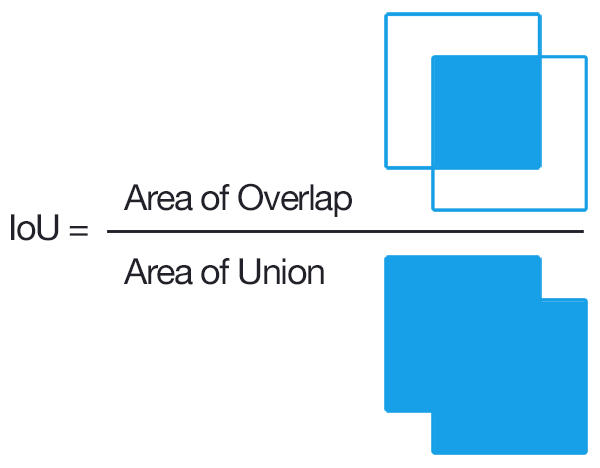
\includegraphics[scale=0.5]{figures/chap222_iou.png}
	\caption{Intersection over Union. The \textit{area of overlap} represents the intersection of the GT with the made prediction. The \textit{area of union} represents the amount of the total area of GT and prediction \cite{Sha18-DLCV}.}
	\label{fig:ch2:sec2:iou}
\end{figure}

An advantage is the inclusion of \textit{false positives} and \textit{false negatives} into the IoU calculation.
A limitation of the IoU metric is that the correctness of the segments boundaries is not taken into account, as discussed in \cite{Csu13-EvalMetric}. 
For this issue they suggest to combine the IoU with another complementary metric, evaluating the boundary of a segment.
Regardless the IoU is a suitable and commonly used metric for semantic segmentation.



\subsection{Architecture}\label{ord:ch2:sec2:subsec3}
The established network architectures for the task of image classification follow a common scheme: 
An input image with lots of features is processed and continuously downsized to make only one prediction.
% For image classification there are established architectures that follow one scheme deep neural networks (DNN) with many layers as \eg VGG-16 \cite{SZ15-VGG16}.
% While processing the input image feature maps continuously get smaller, because only one class is predicted.
In contrast, for semantic image segmentation a class is predicted for each pixel of the image.
Therefore some kind of enlargement in the architecture is required to enable the model to make that high amount of predictions.
% To make this kind of prediction possible, also a reinvention in architecture was required, that enables the model to make that high amount of predictions.
In the following important architectures and their characteristics are examined.

\subsubsection{Encoder-Decoder-Architecture}
The Encoder-Decoder-Architecture as its name anticipates is based on two main parts: the encoder network and the decoder network, visualized in Figure \ref{fig:ch2:sec2:encoder-decoder}.

The encoder network is very similar to a CNN.
It consists out of convolution and pooling layers, that reduce the size of the feature maps and extract features.
The encoder networks of the DeConvNet \cite{NHH15-DeConvNet} and the SegNet \cite{Bad17-EncoderDecoder} even mostly include parts of a popular CNN, the VGG-16 \cite{SZ15-VGG16}. 
In this context the process of applying the encoder network is also called \textit{downsampling}, due to the size reduction of the feature maps.

The decoder network is the counterpart of the encoder network.
It reconstructs the feature maps to their original size, which is also referred to as \textit{upsampling}.
To reach this original size often a reversed architecture of the encoder network is used.
The elemental components of this reconstruction are the operations \textit{unpooling} and \textit{transpose convolution}.

After the encoder network a generally a softmax classifier is applied, that creates a prediction in the form of a probability map.
% probability map with K channels, one channel per class k

% We can observe that coarse-tofine object structures are reconstructed through the propagation in the deconvolutional layers; lower layers tend to capture overall coarse configuration of an object (e.g. location, shape and region), while more complex patterns are discovered in higher layers. Note that unpooling and deconvolution play different roles for the construction of segmentation masks. Unpooling captures example-specific structures by tracing the original locations with strong activations back to image space. As a result, it effectively reconstructs the detailed structure of an object in finer resolutions. On the other hand, learned filters in deconvolutional layers tend to capture class-specific shapes. Through deconvolutions, the activations closely related to the target classes are amplified while noisy activations from other regions are suppressed effectively. By the combination of unpooling and deconvolution, our network generates accurate segmentation maps \cite{NHH15-DeConvNet}.


Representatives of the encoder-decoder-architecture are among others the U-Net \cite{RF15-U-Net}, the DeConvNet \cite{NHH15-DeConvNet} and the SegNet \cite{Bad17-EncoderDecoder}.
\cite{SZ15-VGG16}
\begin{figure}
	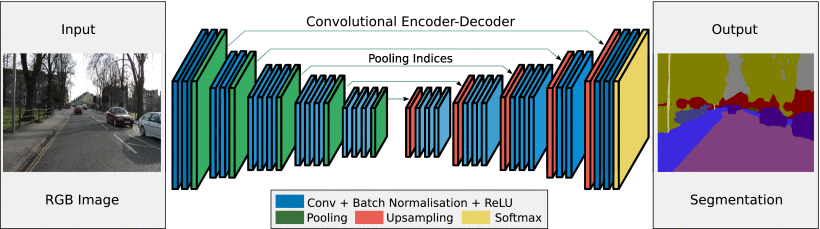
\includegraphics[width=\linewidth]{figures/chap223_SegNetArch.png}
	\caption{Encoder-Decoder-Architecture \cite{Bad17-EncoderDecoder}. On the left the encoder network, which reduces the size of the feature maps while processing. On the right is the decoder network, which reconstructs the feature map to the size of the original input. The yellow layer on the very right is the classification layer, here represented as softmax layer to create the output segmentation.}
	\label{fig:ch2:sec2:encoder-decoder}
\end{figure}

\paragraph{Unpooling}
\cite{Li17-StanfordLecture}
\cite{NHH15-DeConvNet}

\paragraph{Transpose Convolution}
\cite{Dum18-ConvolutionArithmetic}

\begin{figure}
	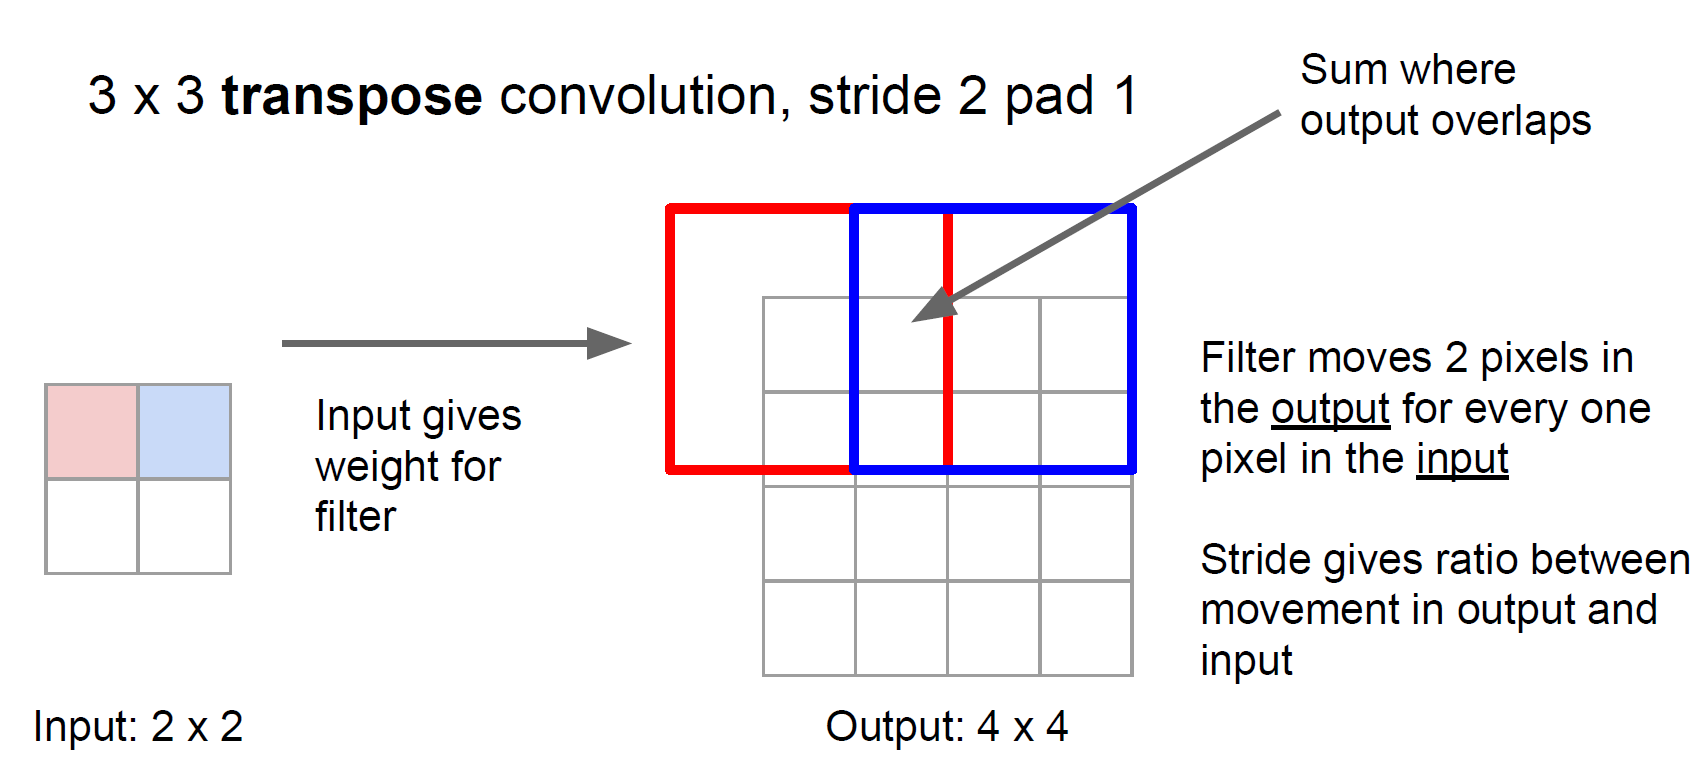
\includegraphics[width=\linewidth]{figures/chap223_TransposeConv.png}
	\caption{tbd}
	\label{fig:ch2:sec2:transpose-conv}
\end{figure}

\subsubsection{Fully Convolutional Networks}
\cite{LSD15-FCN}
\begin{figure}
	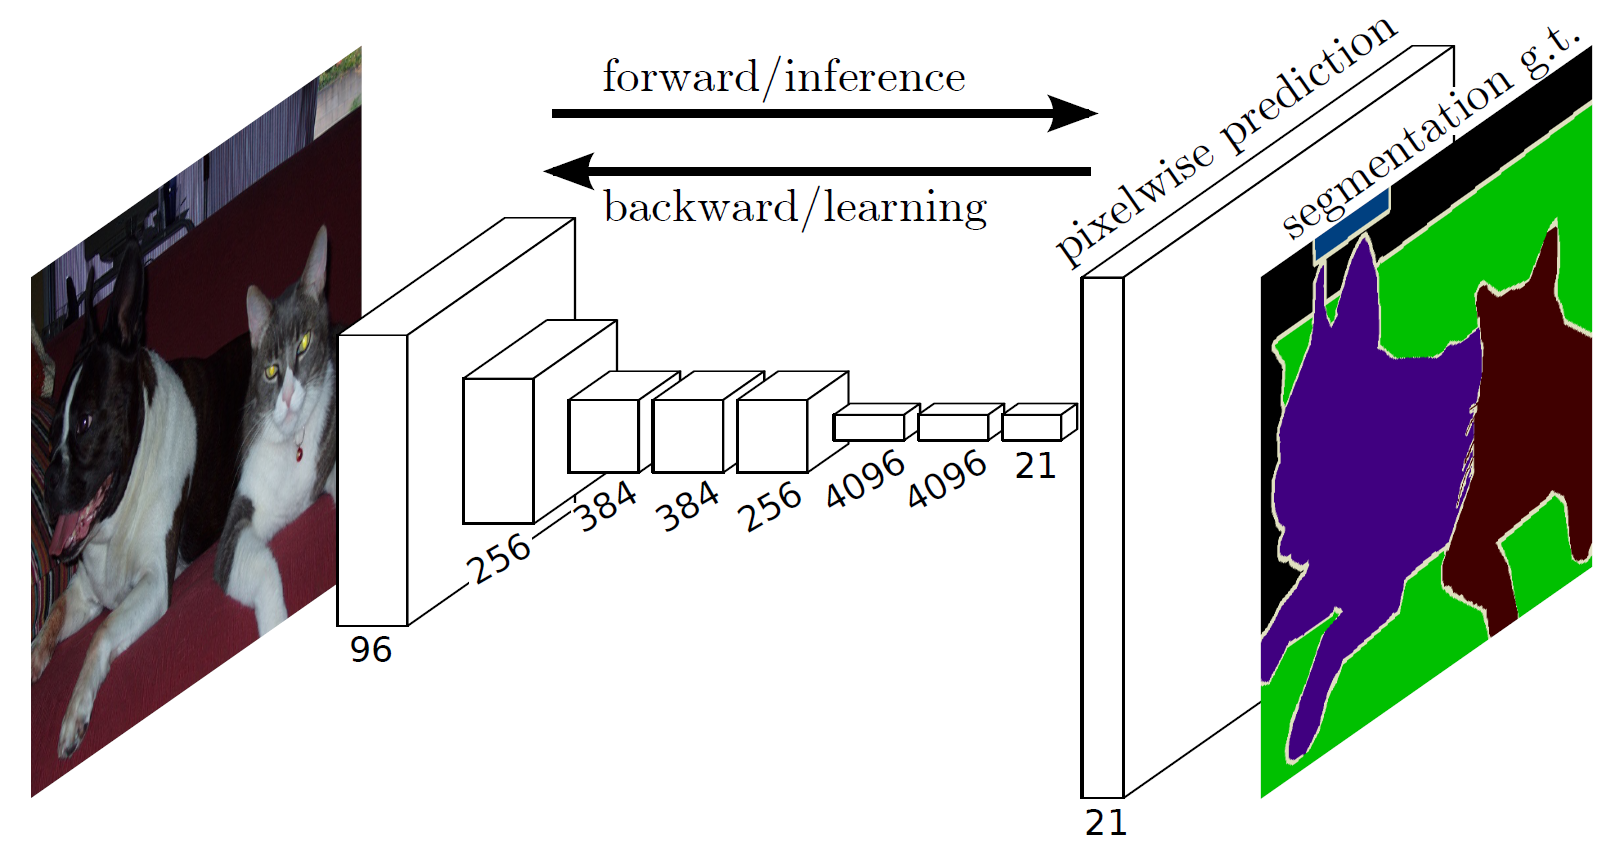
\includegraphics[width=\linewidth]{figures/chap223_FCN.png}
	\caption{tbd}
	\label{fig:ch2:sec2:fcn}
\end{figure}

\paragraph{CRF}
% \cite{Chen16-DeepLab}  --> Atrous Convolution, and Fully Connected CRFs
\cite{Chen16-DeepLab}
\cite{KK12-CRF}


\paragraph{Atrous Spatial Pyramid Pooling}

% \paragraph{Atrous Convolution}

\subsubsection{Lateral connections}
\cite{RF15-U-Net}
\begin{figure}
	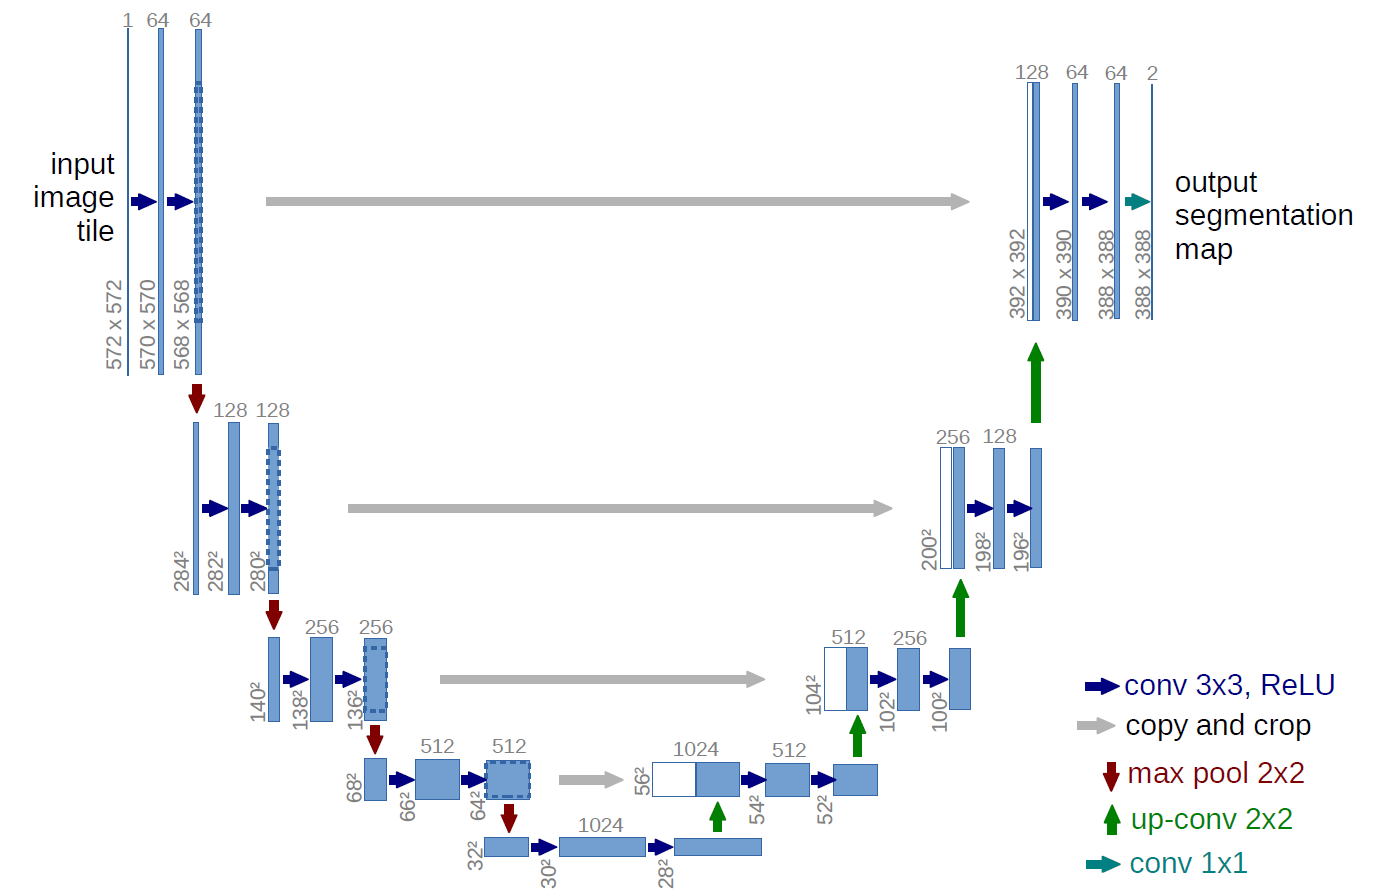
\includegraphics[width=\linewidth]{figures/chap223_Unet.png}
	\caption{tbd}
	\label{fig:ch2:sec2:unet}
\end{figure}



\subsection{Data}\label{ord:ch2:sec2:subsec4}
% TODO introduce GT in Subsec 1
As semantic segmentation is a problem of supervised learning it requires labeled data (GT).
For a dataset to be suitable in the field of DL among others the following criteria should be met: Quantity, quality and representation capabilities.
\begin{itemize}
	% Quantity data - size matters.
	\item The quantity of a dataset used for training a DL model is crucial for its success.
	In general, small datasets, may not cover all vital characteristics to completely map a given objective.
	It has been shown in \cite{Banko01-ScalingData}, that the performance of networks can improve significantly using a larger dataset for training.
	Also, in \cite{Halevy09-UnreasonableEffectivenessOfData} the effect of larger datasets is examined. 
	It is claimed that, using a larger dataset for training can benefit the networks performance more than modifying the architecture of the network \cite{Ger17-HandsOn} \cite{Fer19-SemSeg}.
	This highlights the importance of datasets with sufficient quantity to increase the performance of networks.
	% Quality data.
	\item The performance of a model highly depends on the quality of the training data. 
	Data, that is inconsistent, incomplete, erroneous or too noise, can lead to significant decrease in performance \cite{Gudivada2017-DataQuality}.
	Training with poor quality data makes it more difficult for a model to detect and understand the elemental features and patterns, that are required by a model to perform well \cite{Ger17-HandsOn}.
	% TODO affect of poor quality data for object detection or semantic segmentation. "With respect to the task of semantic segmentation correctness is very significant, for the accuracy of the edges is crucial if a pixel is labelled with the correct class or not."	
	% Representative data.
	\item Another elemental characteristic of a dataset is the representation of the problem, that the corresponding network should solve.
	To enable a model to generalize and perform well, it is essential for the training data to be representative to the problem \cite{Ger17-HandsOn}.
	The best approach to do so, is to include samples of this specific problem or of samples from the same domain.	
	But instead, often general 'all-use-datasets', like Pascal VOC \cite{Eve20-PascalVOC}, COCO \cite{Lin14-Coco} or ImageNet \cite{Deng09-ImageNet}, are applied on a specific problem, that is not covered within the samples of these datasets.
%	For example, the aim of a DL model may be to detect a certain manufacturing part from an industrial scope.
%	But without a dataset that represents this problem well enough, by containing samples from industrial scopes, the performance of the DL model may be significantly worse.
	This may results in a decrease of performance, because the capabilities of DL model are strongly connected with the representation of the data \cite{Goodfellow-et-al-2016}.
\end{itemize} 
% Very hard and expensive to obtain data for semantic segmentation and special domains.
It can be a challenge to obtain a dataset, that meets these criteria.
The creation of new image datasets can be considered very expensive in time and cost.
Datasets for semantic segmentation are even more difficult to create due to the high effort required to label images on pixel-level.
Especially, datasets that cover uncommon or even restricted domains (e.g. medical or industrial domain) are rare to find.
For example, the manufacturing process in a closed industrial environment may contain unique objects or uncommon surroundings, that are hardly ever represented in common datasets.

% New ways to obtain GT -> Labeltool, Interactive methods, AI-Simulation 
To facilitate the process of creating a new dataset and label images with pixel-level accuracy, new approaches have been created.
An efficient and common way is a program, that simplifies the process of labeling by providing an user interface and multiple methods to create and save label.
These programs are often called \textit{Labeltools} or \textit{Annotation tools} and due to the high demand on labeled training data there are various Labeltools available \cite{Cer20-AnnotationsTools}.
To simplify the quite manual labeling process for a human user there are interactive methods (see Chapter \ref{ord:ch2:sec3}), that support the applicant to create a label.
Another approach is to create synthetic datasets like the SYNTHIA dataset \cite{Bengar2019-Temporal} and use them to as training data for semantic segmentation \cite{Chen18-SyntheticData}.


\subsection{State-of-the-art}\label{ord:ch2:sec2:subsec5}
\subsection{Application}\label{ord:ch2:sec2:subsec6}
Semantic Segmentation finds application in various tasks and is widely used over different domains.
Due to its capability to perform classification on pixel-level it is applied on scene understanding \cite{LiJ09-SceneUnderstanding} or the evaluation of satellite images \cite{Li18-SateliteImagery}.
In the field of autonomous driving Semantic Segmentation is used for street scene analysis \cite{Cor16-Cityscapes} \cite{Men15-AutonVehicles} \cite{Neu17-MapillaryDataset}.
In medicine this method can be used to segment blood cells \cite{Tran19-BloodCell}.
Or it is applied in order to fulfill abstract tasks like the reconstruction of indoor scenes \cite{Dai17-ReconstructionIndoorScenes}.
This listing of only some applications gives an idea of how versatile and functional Semantic Segmentation is and what can be achieved with it in the future.